\chapter{移动多摄像头视频自动剪辑}
随着移动设备的普及,很多用户几乎可以在任何时间任何地点拍摄视频记录他们经历的事件。
虽然这些大众化的移动视频被上传到云端或者分享到社交网络,由于视频角度的单一,内容冗余,
声音嘈杂等问题,它们的观看体验十分有限。本章提出一个全自动移动多摄像头视频自动剪辑系统,
可以将同一事件中,多个摄像头从多个角度拍摄的时间上有重叠的一组视频剪辑成内容丰富,
能体现专业编辑水平的单一音视频流。我们通过用户调研总结了一系列可计算的视频编辑规则。
基于这些规则,给定某一事件的一组移动多摄像头视频,我们的系统通过音频指纹同步这些视频,
评价音视频质量,检测视频切换点,并生成音视频流的剪辑结果。音频剪辑在\emph{最小切换准则}
下最大化音频质量得到,视频剪辑最大化视频质量和多样性,同时满足镜头的运动一致性。
我们的系统具有区别于已有系统的三个特点:1)我们的系统能够全自动地完成移动多摄像头自动剪辑;
2)系统引入了从用户调研中总结的一系列视频编辑领域可计算的规则;3)除了视频编辑,
我们考虑了目前系统经常忽视的音频自动剪辑,对于提升用户体验十分重要。
实验评价结果显示我们的系统大的哦了比目前最好的视频自动剪辑系统更好的效果,提供了
更好的用户体验。

\section{主要挑战}
多摄像头视频是指在某一事件中,
由多个用户从多个角度拍摄的时间上有重叠的一组视频~\cite{DBLP:conf/mm/ShresthaWWBA10}。
多摄像头视频的观看体验十分有限。首先,为了对整个事件有全面的了解,依次观看所有视频
十分的耗费时间,由于单个视频的角度单一,用户的观看过程会十分枯燥乏味。其次,不同用户
拍摄的内容可能十分类似,使得它们非常不利于收藏或分享。再次,移动多摄像头
视频主要由业余用户在移动环境下拍摄的,视频的质量无法得到保证。为了这些困难,
移动多摄像头视频自动剪辑将这些移动视频同步,并在不同的时间段只选取一个视频,将一组
视频剪辑成一个内容丰富,看上去具有专业编辑水平的单一音视频流。
图~\ref{fig:mashup-illustrate}是典型的移动多摄像头视频自动剪辑的示意图。
给定某一事件的一组移动多摄像头视频, 我们的系统能够根据一系列剪辑规则生成单一的剪辑音视频流。
每个时间段内选中的视频源在图中用深色表示。自动生成的剪辑视频提供了比任何单一视频更加丰富和更加专业的表达效果,
显著提高了用户体验。
\begin{figure}[ht]
    \centering
    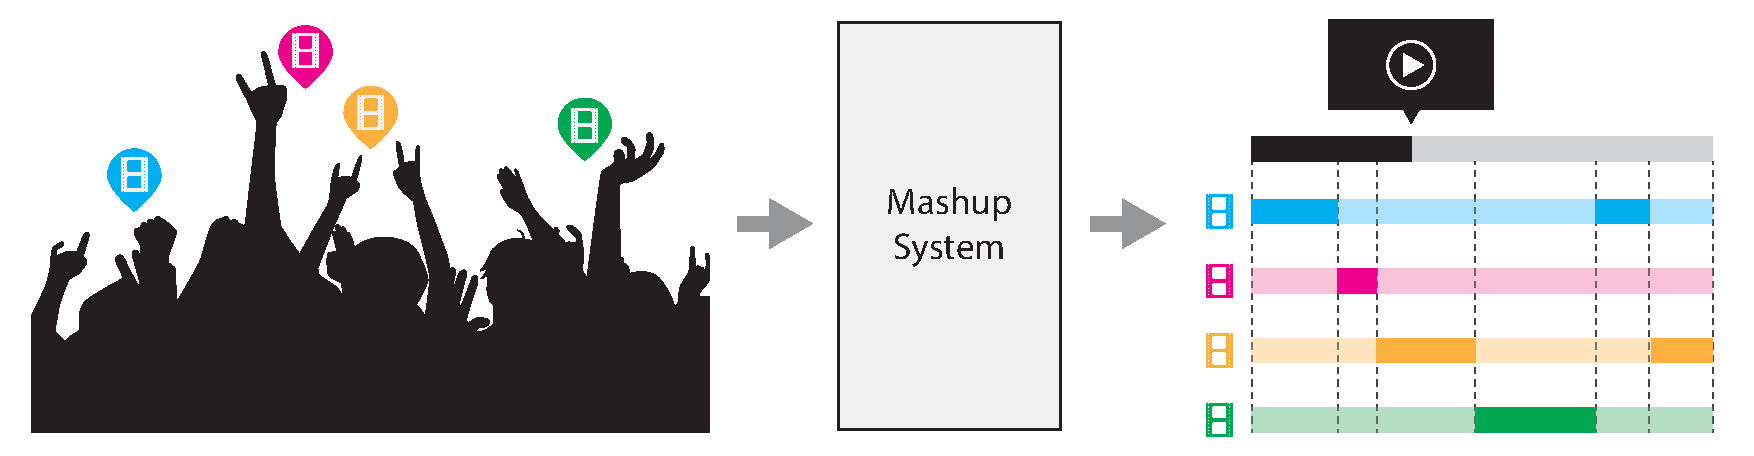
\includegraphics[clip=true, width=0.95\textwidth]{mashup-illustrate.pdf}
    \caption{移动多摄像头视频自动剪辑示意图}
    \label{fig:mashup-illustrate}
\end{figure}

然而,移动多摄像头视频自动剪辑面临这一些困难。第一个困难来自于视频的质量。虽然拍摄设备
已经获得了巨大的发展和提升,视频质量依然会受到抖动,模糊以及拍摄过程中其它因素的影响。
此外,音频质量还受到周围环境以及麦克风本身的影响。据我们所知,
目前很少有关于非侵入式(non-intrusive)音频质量评估的研究。
另一个困难在于我们并不知道专业的编辑人员怎么进行视频剪辑。不同的编辑人员可能有不同的
编辑风格,使得很难学习到通用的模型进行视频剪辑。即使我们了解到人工视频编辑的过程,
我们仍然需要需要将编辑的过程转化成可计算的表达,
这个转化过程也是克服视频剪辑两个基本问题的关键:
何时是从一个音频/视频源切换到另一个的合适时机?如何在所有的音频/视频源
选择最佳的源?

\section{可计算视频编辑语法}
移动视频自动剪辑和视频编辑密切相关。视频编辑人员运用专业的编辑语法,
通过影片的时间片段,阴影效果以及声音抓住用户的注意力,调动用户情绪,
从而向用户讲述视频所要传达的故事。打个比方,视频编辑语法是指用来表述
视觉形式,声音组合,它们存在和出现的功能,以及播放时的相互关系的一套理论。
因此,视频编辑语法包含运动哦嗯个,声音,图像,颜色,电影符号,编辑,蒙太奇等元素~\cite{manchel1990film}。
电影语法最基本的元素包括镜头,运动和距离(全景,中景,近景)~\cite{CinemaElements1982}。
它们不同的镜头长度,拍摄角度,以及距离远近来传达不同的观感。例如,局部的物体运动
可以通过中景镜头表达,而近景通常用来表达静态镜头或者缓和运动镜头。

移动视频自动剪辑模仿电影剪辑的过程来传达原始多摄像头视频记录的事件。移动多摄像头自动剪辑中,
剪切点是指镜头之间的边界时间点,镜头选取是指选取合适的视频流。为了创建内容丰富剪辑专业的视频,
首先需要了解电影剪辑语法以及编辑人员如何运用这些语法到实际的剪辑中。

运用电影剪辑的一个主要难点在于电影剪辑并不是严格的准则。
虽然已经有大量的工作讨论电影语法,本文的部分的结论也不是新的发现,
总结已有的电影编辑规则,发掘新的与移动多摄像头视频剪辑相关的并且方便转化成
可计算规则的电影语法仍然十分必要,这也是本章提出的系统的基础。我们调研了已有的
关于视频编辑的用户调研和论文,并进一步组织了关于视频剪辑的两个基本问题的用户调研:
\begin{itemize}
    \item \textbf{镜头/录音切换}:何时该切换到另一个音频/视频源?
    \item \textbf{镜头/录音选取}:如何选择将要切换到的音频/视频源?
\end{itemize}

\subsection{用户调研}
我们邀请了以为艺术设计领域的教授和一名电影摄影专业的研究生参与了我们的用户调研。
该教授有20多年的视频相关的领域的研究和从业经验。
该研究生有着丰富的视频编辑经验尤其是和电视台的长期合作经验。

用户调研以讨论的形式进行。我们首先展示了典型的拍摄场景(如演唱会,比赛)移动多摄像头
视频的主要问题(光照,抖动,遮挡等等)。我们向他们解释移动多摄像头视频剪辑的含义并
咨询与之相关的问题。这些问题包括:
\begin{itemize}
    \item \emph{视频剪辑讨论}:该讨论主要调研切换频率和镜头选取。我们咨询的问题包括:
        视频镜头的时长是否有要求?哪些因素会影响到镜头时长?它们是如何影响的?
        这些因素与时长之间是否有确定的联系?镜头切换有那些要求?哪些因素跟视频质量密切相关?
        如何避免移动多摄像头视频的单一性问题?如何能够平滑地切换视频镜头?是否有提高观看
        体验的建议?
    \item \emph{音频剪辑讨论}:该讨论主要是关于音频的选取,问题包括:何时需要从一个
        音频源切换到另一个音频源?什么样的音频是比较好的?视频剪辑和音频剪辑之间的差异
        是什么?不同音频源的片段之间如何拼接?
\end{itemize}

\subsection{视频剪辑调研结果}
\label{sec:video-mashup-survey}
\textbf{镜头切换}。两个编辑人员认为他们视频镜头的时长应该有个范围,
太短的镜头内容表达不完整,太长的镜头则显得枯燥。镜头时长不是一个固定的常数值。
Shrestha等人选取的演唱会视频镜头的长度为3秒到7秒。然而,镜头时长也不是严格固定的,
更长的镜头可以用于运动镜头或者定场镜头,因为运动镜头不断拍摄新的内容,防止了内容的
枯燥性,而定景镜头展示了完整的场景和丰富的内容,也不会产生内容单一引起的枯燥性。

镜头切换的频率跟音频和视频都比较相关。较高的切换频率适用于较快的音频节奏,剧烈的物体运动,
以及快速的光照变化,平缓的镜头适宜配以较少的镜头切换。镜头切换频率和这些影响因素之间没有
明确地关系,采用线性关系或者非线性关系取决于编辑者的编辑风格。

合适的切换点应该选择在说话或者歌唱的间歇。开始说话或者唱歌能够抓住观看者的注意力,
并在结束时释放。为了避免打断观看者的注意力,在说话或者唱歌的间歇切换通常是比较好的选择。

\textbf{镜头选取}。与镜头选取相关的可计算的因素包括:视频质量,多样性,相机运动,和语义
完整性。
\begin{itemize}
    \item
        \emph{视频质量}。视频质量保证了视频的清晰度和观看体验的愉悦性。有关视频质量的发现
        包括:太暗或者太亮镜头应该被排除;应避免模糊的镜头;遮挡的镜头会破坏用户兴趣;
        倾斜镜头多数情况下会让观看者感到不适,虽然特殊情况下能够达到特殊的表达效果。
        两位参与者还特别提到由不规律的或者不专业的相机运动引起负面效果(如手的抖动,
        快速运动等)的镜头必须排除。
    \item \emph{多样性}。多样性表示对事件丰富的表达。根据调研,
        视频剪辑中没有明确的准则用来选择相机的角度和距离。
        不同的剪辑人员有不同的剪辑风格,因而在有多个镜头可选时可能也会做出不同的选择。
        然而,镜头选取中也有一些不能违反的规则。比如,一个关键的准则是避免``\emph{跳切}'':
        拍摄相同主体的两个相邻镜头的拍摄位置不能过于接近。\emph{30度准则}表明相邻镜头
        至少应该有30度拍摄角度的差异,从而避免镜头大量的内容重合。
        当相机位置不确定时,剪辑人员推荐应当选择镜头使得帧与帧之间的差别足够大,给观看者
        呈现新的内容。
    \item \emph{相机运动}。为了良好的观看体验,相邻镜头的相机运动应该尽量平滑,
        意外的相机运动会导致令人厌烦的视觉影响。一些通用的准则包括:1)静态镜头应该与
        静态镜头连接;2)运动镜头不适宜放置一起;3)可以通过减慢的相机运动消除运动镜头和
        静态镜头链接导致的部分视觉影响。
    \item \emph{语义完整性}。两位参与者提到一些视频剪辑语义上的一些考虑。
        每个用户拍摄的视频都是有一系列语义完整的部分(后文中我们称之为子镜头)部分构成的。
        视频剪辑不应该破坏每个语义完整的部分,切换时应该选取语义完整的镜头,
        否则,镜头切换会显得十分突兀。
\end{itemize}

\subsection{音频剪辑调研结果}
不同与视频剪辑,音频切换的次数应该越少越好,我们称之为\emph{最小切换准则}。在音频剪辑中
不存在一直播放同一音频源导致的单一性问题。相反,即使多个视频之间在时间上精确同步,
由于音频的音量音色的差异,连接不同的音频源会导致不连贯的问题。这种不连贯性既有可能是
麦克风本身也有可能是录音时的周围环境引起的,使得剪辑音频质量下降。因此,音频剪辑更倾向
于从一个或少数几个音频源创建单一音频流。考虑到移动拍摄环境,应该避免嘈杂的音频,选择
声音清晰干净的音频片段,音频剪辑应该具有鉴别高质量的音频片段的能力。

\subsection{可计算视频编辑语法}
根据用户调研,我们对可计算的电影语法做了总结。这些语法构成了本章节提出的系统的基础。
\begin{itemize}
    \item 对于视频切换点检测,需要满足以下条件:1)镜头时长应该在一个范围之内;
        2)镜头切换的频率应该与音频的节奏想匹配;
        3)切换点应该选择在说话或者唱歌的间歇。
    \item 视频镜头选取应该满足一下准则:1)镜头应该清晰稳定(没有模糊,
        遮挡,抖动等问题);2)相邻镜头之间的帧差应该较大避免\emph{跳切};
        3)切换点附近的相机运动应该平滑自然;4)每个被选择的镜头语义上应该完整。
    \item 音频剪辑应该满足:1)音频片段清晰干净;2)满足\emph{最少切换准则}:音频
        切换的次数应该越少越好。
\end{itemize}

\section{移动多摄像头视频自动剪辑系统}
基于以上总结的可计算的电影准则,本章提出MoVieUp系统用于解决移动多摄像头视频自动剪辑。
后续章节中,视频和音频分别表示视觉信号和音频信号,用录像同时表示两个信号。

\subsection{系统框架}
MoVieUp系统包含音频剪辑和视频剪辑两个部分。为了更清晰地阐述系统原理,我们定义
以下术语:
\begin{itemize}
    \item \emph{镜头}:镜头表示作为剪辑后的视频一个部分的来自于同一个视频源的连续视频片段。
    \item \emph{子镜头}:子镜头是包含连续相机运动和独立语义内容的基本视频单元。
    \item \emph{切换点}:切换点是从一个信号源切换到另一个信号源的时间点。需要注意的是,
        在每个切换点,可能有多个信号源作为选择。
\end{itemize}

\begin{figure}[ht]
    \centering
    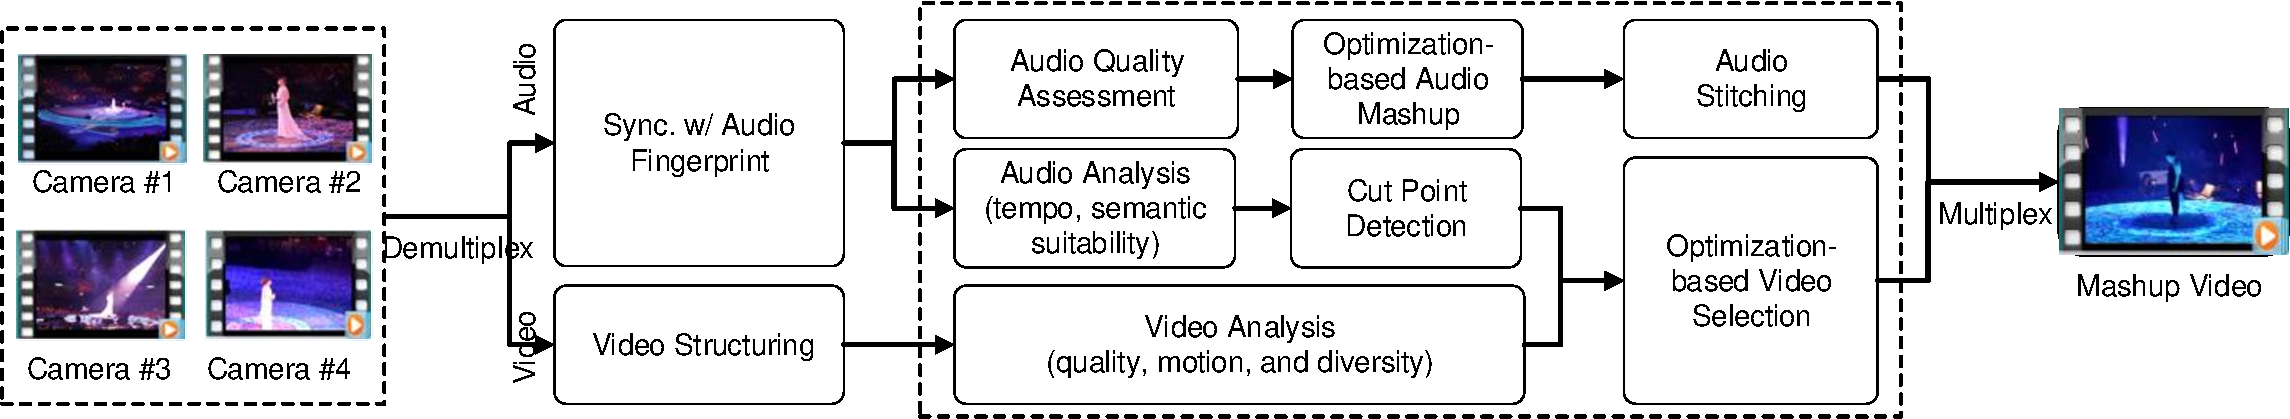
\includegraphics[clip=true, width=0.95\textwidth]{mashup-framework.pdf}
    \caption{移动多摄像头视频自动剪辑系统框架}
    \label{fig:mashup-framework}
\end{figure}
图~\ref{fig:mashup-framework}表示了MoVieUp系统的框架。
给定一组录像,系统将它们分流成音频和视频,在时间上对录像同步,
根据总结的电影语法生成剪辑音频和剪辑视频,并混流成最终的单一音视频流。
对于音频剪辑,我们在\emph{最少切换准则下}根据音频质量选择音频片段。
视频剪辑包含两个步骤:切换点检测和视频镜头选取。系统通过匹配切换频率和音频节奏
在说话或唱歌的间歇检测切换点。给定检测到的切换点,镜头选取定义为保证相机运动一致性
的条件下最大化视频质量和多样性的问题。质量和内容的分析在子镜头的粒度上完成。
系统对视频剪辑的结果进一步微调,从而满足语义完整性。
视频去抖动作为可选的步骤可以进一步提高剪辑视频的观看体验。
系统完成音频剪辑和视频剪辑以后,对两个剪辑结果混流生存最终的结果。

\textbf{符号表示}:假设一共有$N$个录像$\mathcal{R}=\{r_1, r_2, \ldots, r_N\}$。
每个录像$r_i$被分流成音频$a_i$和视频$v_i$。$r_i$开始的时间记为$t_i^{(s)}$,结束的时间记为
$t_i^{(e)}$,$a_i$和$v_i$开始结束的时间与$r_i$相同。第$j$个被选取的音频和视频片段表示为
$s_j^a$和$s_j^v$(第$j$个镜头),相应的时长表示为$d(s_j^a)$和$d(s_j^v)$。
上标$a$和$v$用来区分音频和视频。剪辑后的音频和视频表示为:
\begin{eqnarray*}
	\mathcal{M}^a &= (s_1^a, s_2^a,\ldots, s_{M^a}^a) \\
	\mathcal{M}^v &= (s_1^v, s_2^v,\ldots, s_{M^v}^v).
\end{eqnarray*}

对于视频剪辑,每个镜头最大时长为$d_{max}$,最小时长为$d_{min}$:$d_{min} \leq
d(s_j^v) \leq d_{max}$。切换点$c_j$是视频从$s_{j-1}^v$切换到$s_j^v$的时间点,
对应的时间记为$t_{c_j}$。为了表示方便,事件开始的时间也认为是一次切换点,即
$t_{c_1} = 0$。图~\ref{fig:mashup-symbols}表示了以上符号的含义。
\begin{figure}[ht]
    \centering
    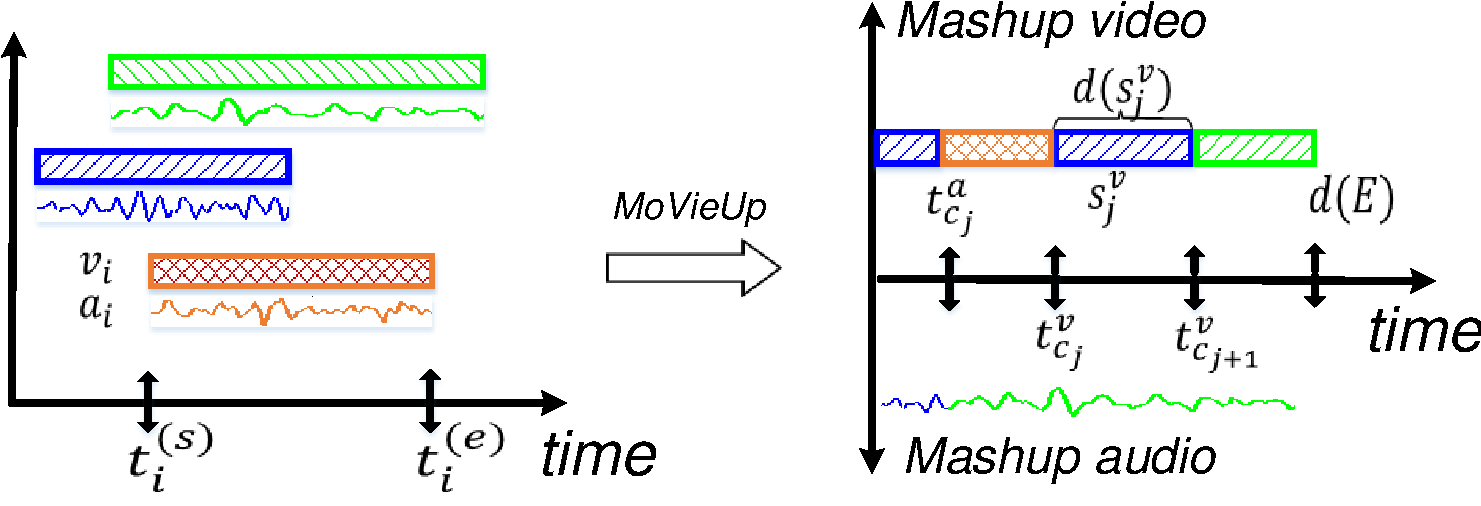
\includegraphics[clip=true, width=0.95\textwidth]{mashup-symbols.pdf}
    \caption{移动多摄像头视频自动剪辑系统符号表示}
    \label{fig:mashup-symbols}
\end{figure}

\textbf{预处理}:系统首先对音视频做预处理,方便后续的分析和优化。
为了同步和质量评估,音频首先被采样到8kHz。视频帧率被采样到25帧/秒,
分辨率被采样到$640\times 360$。

输入的一组录像记录了同一事件的不同时间段。为了进一步的处理,需要将录像在时间上同步,
也就是确定每个录像的起始时间$t_i^{(s)}$和$t_i^{(e)},\forall r_i \in \mathcal{R}$。
同步的基本假设是在事件的任意时间点至少存在一个录像。MoVieUp采用了
Shrestha等人提出的基于音频指纹的方法对录像进行同步~\cite{shresthabws10}。
我们首先提取每个录像的音频指纹,通过比较计算出每一对录像之间的时间差,
再通过投票的方法决定所有录像之间的时间差。

视频和音频剪辑都需要满足同步约束:被选取的信号源的开始时间必须早于当前切换点,
结束时间必须晚于当前切换点。
\begin{eqnarray}
    t_{s_j}^{(s)} \leq t_{c_j} \leq t_{c_{j+1}} \leq t_{s_j}^{(e)}
\end{eqnarray}
当不满足上述约束时,对应的信号源将不作为当前切换点的备选信号源。

对于视频的处理有三个粒度:帧,子镜头和镜头。如同Mei等人分析~\cite{MeiHZZL07},
帧级别的操作不仅十分耗时,也不利于进一步的内容分析,因为帧并不是视频最具有信息量的
语义单元。镜头是由于用户开始和结束操作引起的物理结构,它持续的时间相对较长,包含的内容
也不一定具有一致性。在本章的剪辑系统中,我们选取了包含连续相机运动和完备语义内容的
子镜头作为基本的视频单元,并采用了Kim等人提出的基于颜色和运动阈值的方法对输入视频
做结构分析,得到视频的镜头和子镜头~\cite{KimCKK00}。

\subsection{音频剪辑}
在多摄像头视频剪辑中,每个录音只记录了整个事件一段时间,
音频剪辑是把所有录音综合起来生成一个事件的单一的完整的音频的过程。本章系统通过
在~\emph{最少切换准则}下最大化音频质量的方法剪辑音频。

根据我们用户调研的结果,音频剪辑的主要目的是最大化选取的音频片段的
整体质量$Q(\mathcal{M}^a)$。由于音频切换会降低音频整体的质量,
$Q(\mathcal{M}^a)$并不是简单的各个音频片段的质量之和。
通过仔细研究,我们发现每个移动设备拍摄的音频质量并不会频繁剧烈的抖动。
基于这个发现,我们将~\emph{最小切换准则}具体化为一个音频切换的一个硬性约束。
用$q_{s_j^a}(t)$表示音频片段$s_j^a$在时间$t$的质量,
仅当其它音频的质量明显好于当前音频时才发生切换:
\begin{eqnarray}
	q_{s_{j+1}^a}{(t)} & > \gamma \cdot q_{s_j^a}{(t)},
	\label{equ:mashup-switch-constraint}
\end{eqnarray}
$\gamma$是音频切换的惩罚系数,在实验中设为$1.2$。

我们采用了贪心算法每隔一秒检查所有备选音频的质量,生成最终的剪辑音频。
音频切换发生在当前音频结束时或者另一个音频的质量明显好于当前音频。

\textbf{音频质量评估}:上述方案需要评估音频的质量。据我们所知,
除了一些在语音信号上的工作~\cite{CampbellJG09},很少有无参考通用音频质量评估的研究。
Li等人将无参考音频质量评估建模为排序学习问题~\cite{LiWCDWW13},该工作也音乐质量评估的第一个工作。
然而,该方法并不适用于本章的音频剪辑场景,
如同方程~\eqref{equ:mashup-switch-constraint}所示,我们需要有意义的音频质量评分。

通常,移动多摄像头视频拍摄的事件中音频信号的主体是说话或者歌唱。
因此在本文的系统中,我们采用了P.563~\cite{RixBKKG06},
一种非侵入式语音质量评估算法评价输入音频的质量。
系统用5秒滑动时间窗评价每秒的音频质量。


为了进一步验证P.563算法是否适用于本文的场景,我们随机选取了
四个移动设备录制的音乐会录音,并下载了对应的音乐,我们称之为参考音频。
我们用P.563算法分别评价这两种类型的音频,质量分数如图~\ref{fig:mashup-audio-example}所示。
图中横轴是时间,纵轴是质量评分(Mean Opinion Score, 简称为MOS)。
左图中是四个移动音频的质量评估结果,右图中是对应的参考音频质量评估结果。
我们可以发现移动音频的质量评分明显低于参考音频的评分,从而验证了P.563
算法在本文场景下的有效性。
在音频剪辑中,我们想要选取如图~\ref{fig:mashup-audio-example}所示的Audio 2
开始阶段那样质量高持续时间长的音频片段。
\begin{figure}[ht]
    \centering
    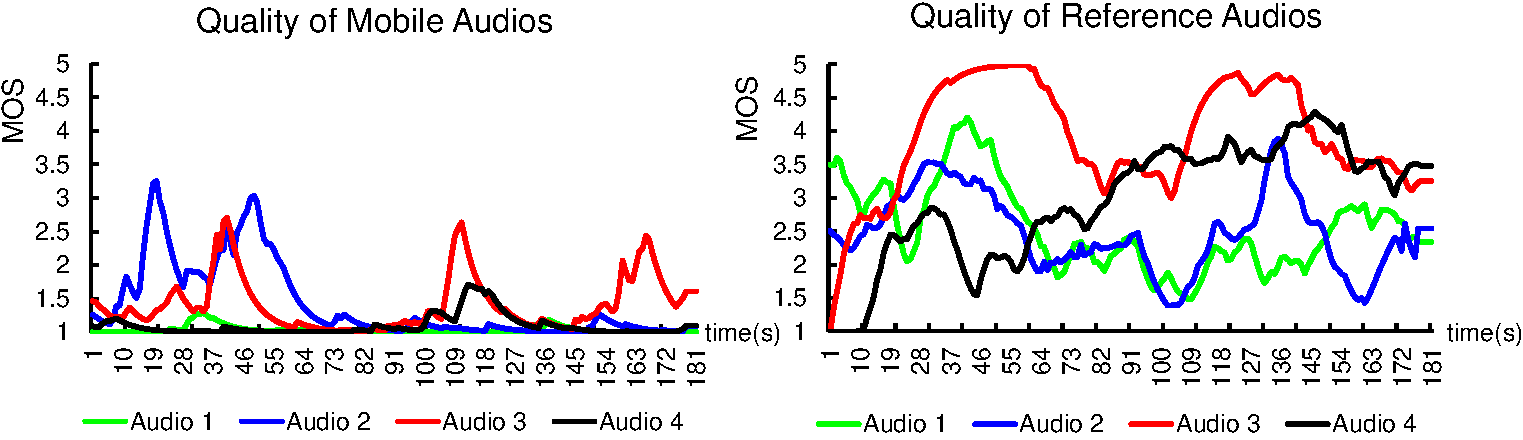
\includegraphics[clip=true, width=0.95\textwidth]{mashup-audio-example.pdf}
    \caption{音频质量评估结果示例}
    \label{fig:mashup-audio-example}
\end{figure}

\textbf{Audio stitching} 选取音频片段以后,系统需要将音频片段拼接成单一音频。
不同与视频,用户对声音的突然变化比较敏感。由于输入的录音是在不同的位置不同的
周围环境下录制的,直接拼接音频片段会导致音量和音色不一致引起的声音突变问题。
为了克服这个问题,我们首先用直流矫正使得音频的音量增益相同,并使用类似与图片融合的基于
拉普拉斯金字塔的算法将音频片段连接到成单一音频。

\subsection{镜头切换点检测}
\label{sec:mashup-cutpoint}
视频剪辑是从输入视频中选取镜头并将他们拼接成内容丰富、具有专业观赏品质的单一视频流。
视频剪辑分为两个步骤:切换点检测和视频镜头选取。本节介绍视频切换点检测,从而决定剪辑视频
应该从一个视频源切换到另一个视频源。

\textbf{建模}:根据电影语法,视频切换点检测需要综合考虑音频(节奏,说话/歌唱间隔)
和视频(相机运动,子镜头完整性等)。MoVieUp系统首先根据剪辑后的音频检测备选的切换点。
对于视频,我们要求在备选的切换点处选取镜头时需要满足运动一致性和语义完整性。
我们提出了两个合适度用于检测视频切换点:节奏合适度($S^T(t)$)和语义合适度($S^S(t)$)。
节奏合适度衡量切换频率和音频节奏之间的关系,语义合适度避免打断说话或歌唱等行为。
切换点检测基于它以前的切换点已经被确定的基本假设,用数学形式表达为:
\begin{equation}
	\begin{aligned}
		t_{c_j} = \argmin_{t}&\big\{{S^T(t|t_{c_{j-1}}) +
		S^S(t|t_{c_{j-1})}}\big\}, \quad s.t. \quad
		d_{min} &\leq t - t_{c_{j-1}} \leq d_{max}
	\end{aligned}
	\label{equ:mashup-cut-pint-detection}
\end{equation}

\textbf{节奏合适度$S^T(t|t_{c_{j-1}})$}:视频切换频率应该与音频节奏相匹配。快节奏的音频
应该配以频繁的镜头切换,低频镜头切换更适合用在节奏缓慢的事件中。我们用音频起始点(onset)
之间的间隔近似音频节奏~\cite{DBLP:conf/mm/HuaLZ03,stowell2007adaptive}。
如同在~\ref{sec:video-mashup-survey}章讨论的,音频节奏和切换频率之间没有明确的关系。我们将时刻$t$的节奏$b(t)$
线性地映射到预期时长$d(b(t))$:
\begin{equation}
	d(b(t)) = d_{max} - \frac{d_{max} - d_{min}}{b_{max} - b_{min}} (b(t) - b_{min}),
\end{equation}
其中$b_{max}$和$b_{min}$分别是最大和最小音频节奏。

$t$时刻的节奏合适度定义为:
\begin{equation}
	S^T(t|t_{c_{j-1}}) = |\int_{t_{c_{j-1}}}^{t}{\frac{1}{d(b(t))}dt} - 1|.
\end{equation}

\textbf{语义合适度$S^S(t|t_{c_{j-1}})$}:语义合适度$S^S(t)$表示我们应该避免让镜头切换
分散用户的注意力。我们通过选择音频能量较低的时间点如说话和歌唱的间隔作为切换点达到这个目的。
语义合适度通过归一化到$[0,1]$范围内的音频能量$e(t)$衡量:
\begin{equation}
	S^S(t) = e(t).
\end{equation}

\textbf{求解}:目标方程~\ref{equ:mashup-cut-pint-detection}是一个连续函数,由于
节奏合适度和语义合适度都不是平滑函数,很难求出该目标方程的闭合解。因此,我们将时间
数字化,步长为$\delta$秒,系统枚举从上一个切换点开始的$[d_{min},d_{max}]$范围内的
所有可能时间点,目标方程的求解转化为:
\begin{equation}
	\begin{aligned}
		t_{c_j}   &= t_{c_{j-1}} + K\delta, \\
		where \quad K &= \argmin_{K}\big\{S^T(K) + S^S(K)\big\},\\
		S^T(K)  &= \big|\sum_{k=1}^K{\frac{\delta}{d(b(k))}} - 1\big|, \\
		S^S(K)  &= e(K)= e(t_{c_{j-1}^v}  + K\delta), \\
		b(k)    &= b(t_{c_{j-1}^v}  + k\delta).\\
	\end{aligned}
\end{equation}

在理想情况下,$\delta$的值应该尽可能小,从而逼近连续的目标方程。
为了选取合适的$\delta$值,我们随即选取了一些音频并用不同的$\delta$取值检测切换点。
图~\ref{fig:mashup-cut-point}显示了其中两个随机选取的音频检测结果。
我们发现当$\delta$小于$0.2$秒时,检测到的切换点十分类似。因此,我们在实验中$\delta$
取值为$0.1$。用$d(e)$表示事件的时长,当$d(e)$在几分钟的量级时,
目标方程~\ref{equ:mashup-cut-pint-detection}需要枚举的时间点个数为$d(e)/\delta$,
一般不超过几千的量级,因而相应的计算复杂度也在合理的范围内。
\begin{figure}[ht]
    \centering
    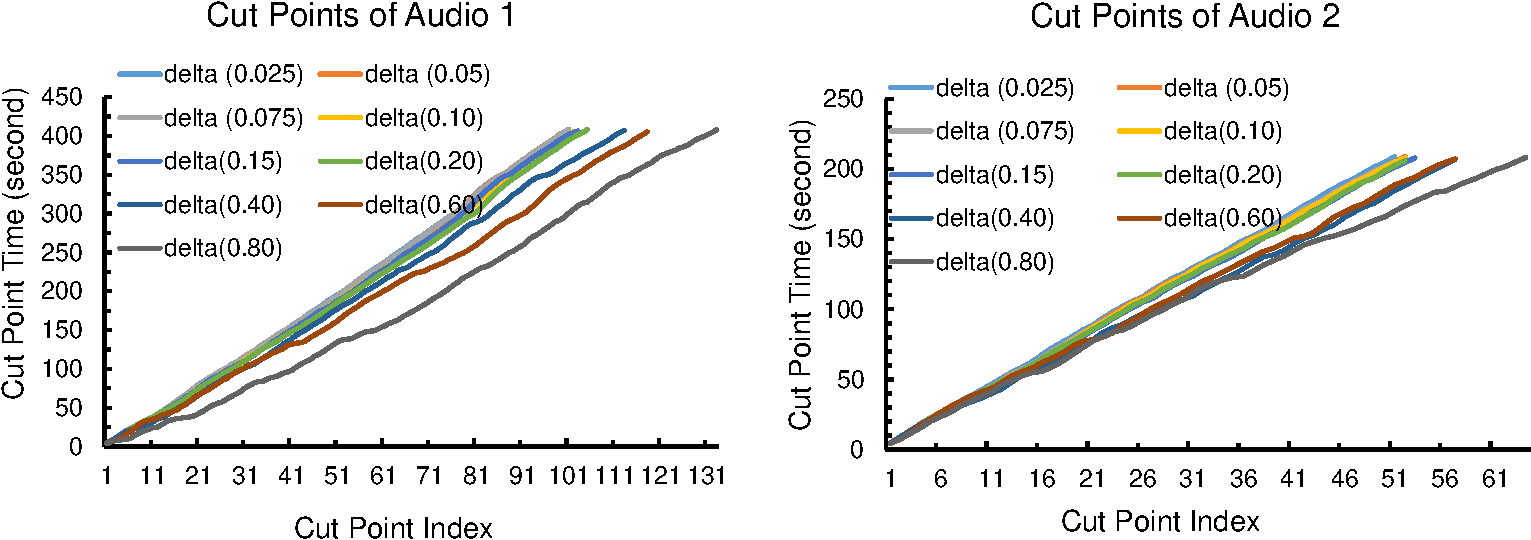
\includegraphics[clip=true, width=0.95\textwidth]{mashup-cut-point.pdf}
    \caption{不同$\delta$取值对视频切换点检测的影响}
    \label{fig:mashup-cut-point}
\end{figure}

\subsection{视频镜头选取}
视频镜头选取是在每个切换点确定如何选取应该切换到的视频源。
本节将视频镜头选取建模为相机运动一致约束下的优化问题。

\textbf{建模}:根据用户调研的结果,视频镜头选取需要综合考虑视频质量,多样性,相机运动和语义
完整性。由于语义完整性依赖被选取的镜头,我们将会在后处理中考虑语义完整性。
因此,视频镜头选取建模为相机运动运动一致性约束下的最大化视频质量和多样性问题。
具体来说,为了简化相机运动一致性的约束,我们禁止切换点附近选取有相机运动的镜头。
该简化方案能达到两个效果:1)减小连接运动镜头带来的视觉冲击;2)平滑相机运动的变化,
因为该约束下相机运动将不会被打断。

用第$j$个被选取的镜头$s_j^v$左右两边的相机运动为$\m^-(s_j^v)$和$\m^+(s_j^v)$,相机运动
一致性表示为:
\begin{equation}
	\m^-(s_j^v) = \m^+(s_{j}^v) = 0,
\end{equation}

用$Q(\mathcal{M}^v)$表示剪辑视频的质量,$D(\mathcal{D}^v)$表示多样性,视频镜头选取
定义为:
\begin{equation}
	\begin{aligned}
		\mathcal{M}^v = \argmax_{(s_1^v, \ldots, s_{M^v}^v)}\big\{Q(\mathcal{M}^v)& + D(\mathcal{M}^v)\big\}, \quad s.t. \\
		\m^-(s_j^v) = \m^+(s_{j - 1}^v) &= 0, \forall j \in [2,M^v].
	\end{aligned}
	\label{equ:mashup-formu-vss}
\end{equation}

\textbf{视频质量评估}:不同与音频,视频质量不会因为镜头切换降低。
视频剪辑的整体质量表示为:
\begin{equation}
	Q(\mathcal{M}^v) = \sum_{j=1}^{M^v}{Q(s_j^v)},
\end{equation}
其中$Q(s_j^v)$是时间段$[t_{c_j},t_{c_{j+1}}]$内镜头$s_j^v$的质量分数。

我们采用了不参考视频质量评估方法衡量移动视频的质量。视频质量从两大类别(时间和空间)
六个方面进行衡量~\cite{MeiHZZL07}。时间因素,包括不稳定性(unstableness)和急动(jerkiness),
是有不规律的相机运动引起的。空间因素,包括失真(infidelity),亮度(brightness),
模糊(blurring) ,倾斜(tilting),是由于恶劣的拍摄环境引起的。我们在子镜头的粒度上
评估六个方面的分数$u_i^v \in [0,1], i \in [1,6]$。
子镜头的不合适分数$U$和质量分数$Q$通过两个步骤计算得到:
\begin{itemize}
    \item 预筛选低质量的子镜头。如果任一子镜头的某个质量分数低于对应的阈值,则认为
        该子镜头不适合被被选取。我们将它的不合适度设为一个较大的值(在实验中设为$1,000$),
        从而保证在该子镜头持续时间内,仅有该子镜头可选时该子镜头仍会被选中。
    \item 基于准则的方法计算子镜头的整体不合适分数$U$和质量分数$Q$~\cite{MeiHZZL07}:
        \begin{eqnarray}
            &U &= E(u^v) + \frac{1}{10 + 6\gamma}\sum_{i=1}^6{(u_i^v -
            E(u^v))}, \nonumber \\
            &Q &= 1 - U,
        \end{eqnarray}
        $E(u^v)$是子镜头六个方面质量分数的平均值。$\gamma$是预先定义的常数值,控制
        $u_i^v$和$E(u^v)$之间的差异对整体分数的影响。
        按照Tao等人在论文中的设定~\cite{MeiHZZL07},$\gamma$取值为$0.20$。
        镜头的质量$Q(s_j^v)$取所有子镜头质量的最小值。
\end{itemize}

\textbf{多样性}:整体多样性是所有选取镜头多样性之和:
\begin{equation}
	D(\mathcal{M}^v) = \sum_{j=1}^{M^v}{D(s_j^v)},
\end{equation}
$D(s_j^v)$是选取的第$j$个镜头的多样性。多样性主要与用户观看过仍停留在记忆中内容有关。
我们根据多大程度上镜头能唤起用户记忆中内容来衡量多样性。$D(s_j^v)$的计算方式为:
\begin{equation}
	D(s_j^v) = D(s_j^v, s_{j-1}^v).
\end{equation}
类似于Sundaram等人提出的记忆模型~\cite{sundaram2002computable},
两个镜头之间的记忆和多样性通过对应相邻的两个子镜头$a$和$b$计算得到:
\begin{equation}
	\begin{aligned}
		R(a,b) &= s(a,b)\cdot f_a \cdot f_b \cdot (1- \frac{\Delta t}{T_m} ), \\
		D(a,b) &= 1 - R(a,b),
	\end{aligned}
\end{equation}
$T_m$是记忆大小。 $s(a,b)$是相邻两个子镜头之间的相似度,
传统方法依赖低层次的特征表达,不能从语义层面解决多样性的问题,
本文收集常见的物体和场景类别,并从社交多媒体网站和搜索引擎收集相关的弱标注数据,
根据本文提出的弱监督深度学习方法,学习这些类别和场景的深度识别网络。
由于深度学习网络的每一层都是对语义不同层次语义的表达,
本文将这些层次的特征拼接到一起组成高维特征,
并利用本文提出的特征选取算法选取最能体现图片语义的特征,
从而获取更好的镜头相似度的计算。
$f_a$和$f_b$是子镜头长度相对于记忆大小$T_m$的比例。$\delta t$是两个子镜头的时长差。

\textbf{问题求解}:为了求解目标方程~\eqref{equ:mashup-formu-vss},我们将约束条件表示成
指示函数$I(s_j^v)$,当约束条件满足时$I(s_j^v)$等于0,否则取一个很大的值作为惩罚项(在我们的
实验中取值为$1,000$),从而保证当且仅当该镜头为唯一选择时才会被选中到最终的剪辑视频中。
目标方程被重新表示为:
\begin{equation}
	\mathcal{M}^v = \argmin_{(s_1^v, \ldots, s_{M^v}^v)}
	\bigg\{ \sum_{j=1}^{M^v}{\big\{U(s_j^v) + I(s_j^v)\big\}}
	+  \sum_{j=2}^{M^v}{R(s_j^v, s_{j-1}^v)} \bigg \}.
	\label{equ:mashup-reformu-vss}
\end{equation}

上述目标方程可以定义成递归的形式。用$f(s_m^v:s_n^v)$表示切换点$m$到$n$(不包括$m$)
上述目标方程的最优值:
\begin{eqnarray}
    f(s_m^v:s_n^v) &=& \min_{(s_{m+1}^v, \ldots, s_{n}^v)}\bigg\{ R(s_{m}^v,
        s_{m + 1}^j) \nonumber \\
        &&+ \sum_{j=m + 1}^{n}{\Big( U(s_j^v) +I(s_j^v)\Big)}
		+ \sum_{j = m + 2}^{n}{R(s_{j - 1}^v, s_{j}^v)} \bigg\}  \nonumber \\
		&=& \min_{s_{m+1}^v}\bigg\{U(s_{m+1}^v) + I(s_{m+1}^v)
		+ R(s_{m}^v, s_{m + 1}^j)
		+f(s_{m+1}^v:s_n^v)\bigg\}, \nonumber \\
		where&& 1\leq m \leq n \leq M^v.
	\label{equ:mashup-recur-vss}
\end{eqnarray}

递归方程~\eqref{equ:mashup-recur-vss}具有最有子结构的特性,为了优化$f(s_m^v:s_n^v)$,
我们首先需要针对每一个可能的$s_{m+1}^v$优化$f(s_{m+1}^v:s_n^v)$。利用该最有子结构
特性以及递归方程,我们可以通过动态规划获得最有解。

假设存在虚拟的唯一初始镜头$s_0^v$并满足所有约束条件。初始目标方程~\eqref{equ:mashup-reformu-vss}
可以利用动态规划和方程~\eqref{equ:mashup-recur-vss}求解方程~\eqref{equ:mashup-vss-final-obj}得到。
\begin{eqnarray}
    \mathcal{M}^v = \argmin_{(s_1^v, \ldots,
    s_{M^v}^v)}{f(s_0^v:s_{M^v}^v)} \nonumber\\
    U(s_0^v) = I(s_0^v) = 0, R(s_0^v, s_1^v) = 0
    \label{equ:mashup-vss-final-obj}
\end{eqnarray}

\textbf{后处理}:根据用户调研的结果,每个录像都是有许多语义完整的子镜头构成的。
上述剪辑步骤没有考虑语义完整性。切换点可能出现在子镜头中间,使得被选取的子镜头可能太短,
破坏了语义完整性。此外,应该进一步减少不规则相机运动引起的抖动,提高用户体验。

因此,我们对剪辑结果进行两步后处理操作:语义完整性和视频抖动矫正。对于语义完整性,我们对切换点附近的
子镜头增加时长的约束,如果某个子镜头持续的时间少于一秒,我们对切换点的位置进行微调使得子镜头
的时长满足约束。对于视频稳定性,我们才用了等人提出的视频抖动矫正方法减小移动视频抖动的影响~\cite{liu2013bundled}。


\section{实验结果}
本节主要评价本章提出的移动多摄像头视频自动剪辑系统的效果。
图显示了移动多摄像头视频剪辑的一个样例。沿着时间轴上方是移动设备录制的备选音频,
波形表示音频的能量曲线。 下方是移动设备拍摄的备选视频,
视频通过每隔30秒采样帧来表示。
系统从这写备选音频/视频中选取片段/镜头生成最终的剪辑音频/视频,
如途中绿色方框所示。
\begin{figure}[ht]
    \centering
    \includegraphics[clip=true, width=0.95\textwidth]{mashup-example.pdf}
    \caption{移动多摄像头视频自动剪辑结果示例}
    \label{fig:mashup-example}
\end{figure}

本实验的主要目的在于从三个准则上对系统进行评估:1)音频剪辑是否提高了最终结果的音频质量,
实验通过与\emph{Virtual Director}系统~\cite{DBLP:conf/mm/ShresthaWWBA10}进行对比,
该系统在选取视频镜头的同时选取对应的音频组成最终的音频输出;
2)与人工选取切换点以及Mukesh等人提出的基于学习的方法~\cite{DBLP:conf/mm/SainiGYO12}相比,
切换点检测算法能达到什么样的效果?
3)本章提出的MoVieUp自动剪辑系统是否提高了移动多摄像头的观看体验?
比较的基准包括两个现有系统:Virtual Director~\cite{DBLP:conf/mm/ShresthaWWBA10}和
Jiku Director~\cite{DBLP:conf/mm/SainiGYO12}。
评价主要从视频的质量,多样性,稳定性和整体的观看体验四个方面进行。

\subsection{数据集}我们从Youtube网站\footnote{\url{http://www.youtube.com}}上收集了6个事件
一共46个录像,也是目前关于移动多摄像头自动剪辑最大的数据集。每个录像包含音频流和视频流。
所有录像都是由不专业的用户通过移动设备拍摄的。上述章节中提到的视频质量问题在数据集中普遍存在。
前三个事件的14个录像与\emph{Virtual Director}使用的数据相同,
我们用\emph{Virtual Director}的作者提供的剪辑视频\footnote{Test videos:
\url{http://www.youtube.com/AutomaticMashup}}作为比较对象。
剩下的32个录像被提交到\emph{Jiku Director}中得到相应的剪辑视频。表格~\ref{tab:mashup-dataset-opt-time}
显示了数据集的详细情况。我们在一台8CPU 16GB
内存的Windows服务器上处理运行MoVieUp系统。平均来说,需要45秒左右的时间评估一分钟
音频的质量。对于一分钟的视频,需要240秒左右的时间做视频结构化分析,65秒的时间做运动分析,
13秒的时间做质量评估。系统优化占用的时间如表~\ref{tab:mashup-dataset-opt-time}所示。

\begin{table}[htbp]
	\centering
	\caption{移动多摄像头视频数据集及算法优化时间}
	\label{tab:mashup-dataset-opt-time}
	\begin{tabular}{|c|c|c|c|c|c|c|}
		\hline
        事件 & 录像数目 & 时长 & 同步 & 音频剪辑 & 切换点检测 & 视频剪辑 \\
		\hline
		E1 & 5 & 4'37'' &1'44''  & 0.11'' & 1.58'' & 26.19''  \\ \hline
		E2 & 5 & 7'01'' &2'38''  &0.14'' & 2.26'' & 36.26''  \\ \hline
		E3 & 4 & 5'15'' &27''  &0.11'' & 1.90'' & 10.26''  \\ \hline
		E4 & 8 & 6'25'' &2'55''  & 0.10'' & 2.11'' & 2'49'' \\ \hline
		E5 & 11 & 3'32''&6'07''  & 0.11'' & 1.36'' & 6'26'' \\ \hline
		E6 & 27 & 5'22''&33'27''  & 0.19'' & 1.90'' & 19'24'' \\ \hline
	\end{tabular}
\end{table}

\subsection{实验设置}
对于音频剪辑评估,我们要求用户听本章算法和\emph{Virtual Director}产生的一对音频,
并做出评分。我们遵循MOS(Mean Opinion Score)的评分策略:
1代表很差,2代表差,3代表一般,4代表好,5代表很好。每个音频对应的系统对于用户是透明的。
每组视频内部的顺序对不同用户都是随机的。

由于普通用户对于视频镜头切换点的敏感性比较低,为了更好地评价视频切换点,
我们邀请了两位专业的视频编辑人员(与用户调研中的参与者不同)评价视频
切换点的合适度。同时我们也邀请两位编辑对切换点给出他们的意见。该评价围绕两个方面开展:
\begin{itemize}
    \item 切换频率是否合适?
    \item 切换点是否出现在合适的时机?
\end{itemize}
我们随机打乱了\emph{Virtual Director}, \emph{Jiku Director}
以及我们系统生成的一共12个剪辑视频的顺序。两位编辑需要依次观看这些视频并
针对上面两个问题给出他们的评分,分数范围与含义与音频剪辑评估相同。

对于视频镜头选取,我们组织了在线用户调研比较不同系统产生的视频的观看体验。
在调研开始前,我们提供了介绍页面帮助用户了解移动多摄像头视频自动剪辑以及用户
即将要完成的评价内容,包括多样性,视频质量,稳定性,和总体评价四个方面,每个方面
的评价围绕着一下问题进行打分:
\begin{itemize}
    \item \textbf{多样性}:视频是否给出了事件丰富的概览?该问题调查剪辑的视频是否
        提供单一的视角使得用户感到厌烦.
    \item \textbf{视觉适量}:视频的视觉质量是否良好?
        此处的视觉质量主要是关于影响质量的空间因素.
    \item \textbf{稳定性}:视频是否稳定?由于抖动是移动视频的主要质量问题之一,
        我们突出视频的稳定性评价.
    \item \textbf{总体评价}:该视频编辑是否专业?
\end{itemize}
用户被要求针对每个视频回答上述四个问题并给出从1(完全不同意)到7(完全同意)的评分.

我们邀请了一位用户体验设计师设计了评价页面。不同于已有系统在实验中依次播放每个视频,
设计师建议我们同时播放两个对比视频,两个视频按图所示分左右两边分别摆放。两个视频的顺序
是随机的。用户需要在不知道视频顺序以及对应的剪辑系统的情况下给两个视频分别打分。
这种评价方式的优点包括:
\begin{itemize}
    \item 用户可以直观地感受到两个视频之间的差异。在已有系统的实验中,
        用户需要记住上一个视频的所有内容和细节。
    \item 同时观看两个视频不会让用户感到迷惑,
        如果同时播放更多的视频会分散用户的注意力。
\end{itemize}
根据以上设定,本章提出的MoVieUp系统在前三个事件上与\emph{Virtual Director}比较,
在后三个事件上与\emph{Jiku Director}比较。
\begin{figure}[ht]
    \centering
    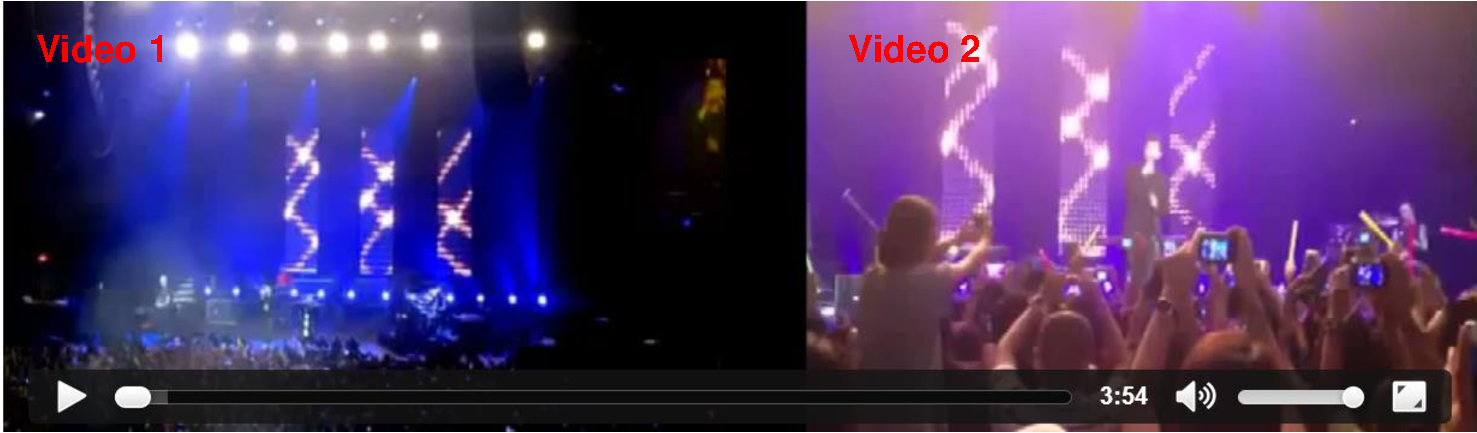
\includegraphics[clip=true, width=0.95\textwidth]{mashup-eval-interface.pdf}
    \caption{视频剪辑评价页面}
    \label{fig:mashup-eval-interface}
\end{figure}

\subsection{音频剪辑评价}
在音频剪辑评价中,我们进行了两组不同设置的实验。
在第一组实验中,我们评价本章提出的音频拼接方式是否有效。由于
MoVieUp系统遵循\emph{最少切换准则},相应的剪辑音频的切换次数也较少(如
表格~\ref{tab:mashup-audio-switch-times}所示)。
因此,我们从三个剪辑音频中选取了30秒切换最频繁的片段作为评价对象,\emph{Virtual Director}
产生的对应时间段的音频用来作为比较。
\begin{table}[htpb]
    \centering
	\caption{剪辑音频的切换次数}
	\label{tab:mashup-audio-switch-times}
	\begin{tabular}{|c|c|c|c|c|c|c|}
		\hline
		\multirow{2}{*}{系统} & \multicolumn{3}{c|}{设定1} &
		\multicolumn{3}{c|}{设定2}\\
		\cline{2-7}
		& 音频 1& 音频 2 & 音频 3 & 音频 4 & 音频 5 & 音频 6 \\
		\hline
		MoVieUp &\textbf{1} &\textbf{2} & \textbf{1} & \textbf{2} & \textbf{1}& \textbf{4} \\
		\emph{VD} &5 & 5 & 4 & 86 & 23 & 76 \\
		\hline
	\end{tabular}
\end{table}

我们邀请了18名用户(包括14名男性和4名女性)参与用户调研。用户年龄在22岁到26岁之间。
其中,观看视频录像(演唱会,比赛,等等)的频率分布为:几乎不看--2人,每月--3人,
 每周--6人,每天--7人。评价结果如表格~\ref{tab:mashup-audio-eval}所示。
 本章提出的音频拼接方法可以有效地减少音频切换带来的听觉影响,
 尤其在音频的音量和音色差异较大时(音频2)时改善更加明显。
\begin{table}[htpb]
	\centering
    \caption{音频剪辑主观评价(MOS)}
	\label{tab:mashup-audio-eval}
	\begin{tabular}{|c|c|c|c|c|c|c|}
		\hline
		\multirow{2}{*}{系统} & \multicolumn{3}{c|}{设定1} &
		\multicolumn{3}{c|}{设定2}\\
		\cline{2-7}
		& 音频 1& 音频 2 & 音频 3 & 音频 4 & 音频 5 & 音频 6 \\
		\hline
		MoVieUp &\textbf{2.56} &\textbf{2.28} & \textbf{3.56} & \textbf{3.00} & \textbf{3.81}& \textbf{3.0} \\
		\emph{VD} &2.33 & 1.28 & 3.5 & 1.75 & 2.81 & 2.38 \\
		\hline
	\end{tabular}
\end{table}

在第二个设定中,我们评价另外三个剪辑后的完整音频。该设定的目的是确认本章的音频剪辑方法是否能够提高
音频剪辑的质量。我们邀请了另外16名用户,包括5名女性和11名男性,年龄分布从20岁到33岁。
观看视频录像的频率分布为:几乎不看--2人,每月--1人,
每周--10人,每天--3人。根据表格~\ref{tab:mashup-audio-eval}中设定2的结果可以发现,
本章提出的系统剪辑的音频质量比\emph{Virtual Director}要好很多。

根据以上两个设定的实验结果,我们的系统从三个方面生成了更好的剪辑音频:
1)提出了更好的音频选取算法;2)显著减少了音频切换的次数;3)系统更平滑地
拼接各个音频片段,减少了音频切换引起的突兀的听觉效果。

\subsection{切换点检测评估}
本节比较本章提出的切换点检测算法相比于\emph{Virtual Director}以及\emph{Jiku Director}
的效果,其中\emph{Virtual Director}根据所有录像中质量最好的音频人工选取切换点,
\emph{Jiku Director}和MoVieUp系统根据算法自动选取切换点。

\begin{figure}[ht]
    \centering
    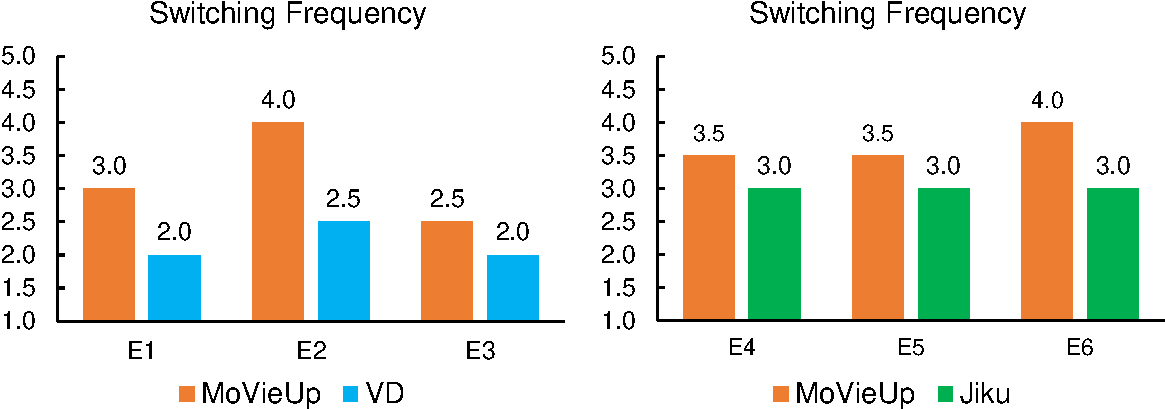
\includegraphics[clip=true, width=0.95\textwidth]{mashup-eval-switching-frequency.pdf}
    \caption{视频切换频率实验比较结果}
    \label{fig:mashup-eval-switching-frequency}
\end{figure}
图~\ref{fig:mashup-eval-switching-frequency}显示了切换频率的实验比较结果。
MoVieUp系统的切换点频率明显优于\emph{Virtual Director}系统。考虑到\emph{Virtual Director}
通过人工选取的方法获得切换点,我们与编辑人员讨论发现\emph{Virtual Director}
选取了很多无意义的切换点。这些无意义的切换点是由于视频中出现了负面效果(抖动,遮挡等)引起的。
虽然我们的系统同样音频中选取视频切换点,它在视频质量方面表现的更好,从而避免了无意义的切换。
编辑人员提醒我们当没有合适的视频可供选取时,不切换通常是更好的选择。

\begin{figure}[ht]
    \centering
    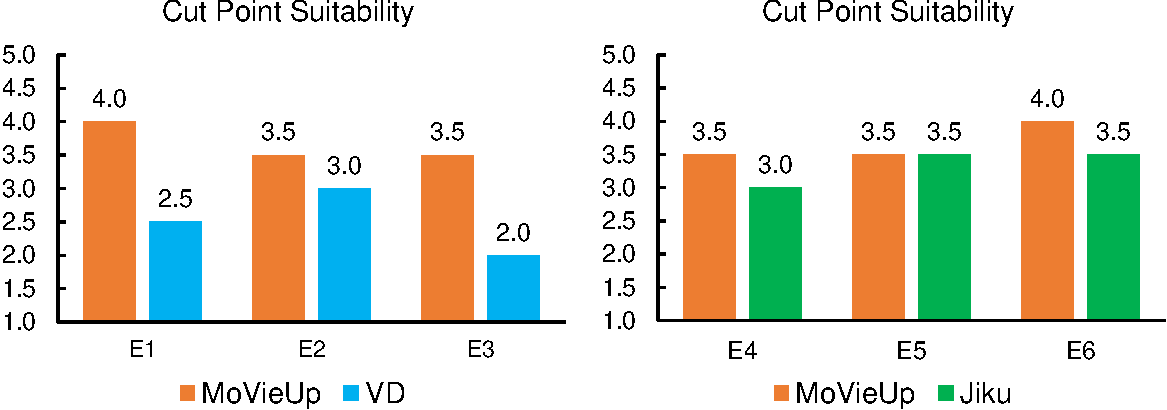
\includegraphics[clip=true, width=0.95\textwidth]{mashup-eval-cutpoint.pdf}
    \caption{视频切换点位置实验比较结果}
    \label{fig:mashup-eval-cutpoint}
\end{figure}
视频切换点位置合适度的比较结果如图~\ref{fig:mashup-eval-cutpoint}所示。
同样由于无意义的切换点的原因,\emph{Virtual Director}获得了很差的评分。
该结果验证了切换点检测不仅与音频有关,也依赖于视频信息。根据评分,MoVieUp
获得了比\emph{Jiku Director}略好的结果。在用户调研中,
编辑人员推荐在说话或歌唱等语义行为的间隔切换,我们也发现部分文献建议在音乐的节奏点切换,
编辑人员也很难给出明确地切换点选取规则。即使如此,试验结果仍然表明MoVieUp提供了一个
可行的切换点检测方案,检测结果达到了\emph{一般}甚至\emph{好}的评价级别。

\subsection{视频剪辑评估}
本节评价本章提出的系统MoVieUp相对于\emph{Virtual Director}和\emph{Jiku Director}
的观看体验。为了公平起见,实验中MoVieUp没有采用视频稳定的后处理措施。

\textbf{与\emph{Virtual Director}的比较}:
我们邀请参与音频剪辑第一组实验的18名参加MoVieUp系统与\emph{Virtual Director}
的比较实验,结果如图~\ref{fig:mashup-comp-vd}所示。
\begin{figure}[ht]
    \centering
    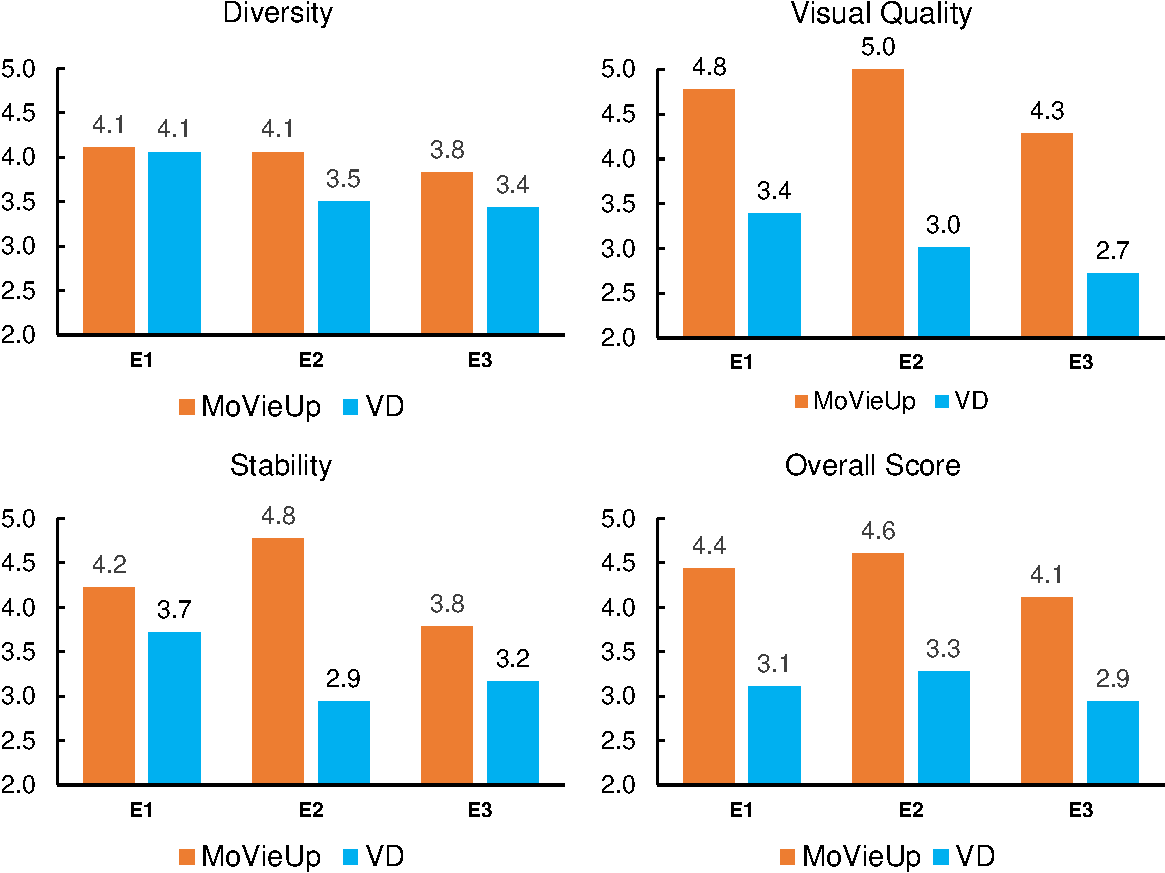
\includegraphics[clip=true, width=0.95\textwidth]{mashup-comp-vd.pdf}
    \caption{MoVieUp系统与\emph{Virtual Director}的实验比较结果}
    \label{fig:mashup-comp-vd}
\end{figure}

我们发现,MoVieUp系统在多样性方面比\emph{Virtual Director}表现更好,
但相对于其他三个评价因素,多样性的优势并不十分明显。该结果也在合理的范围之内,
因为两个系统都在切换点选取不同的视频源避免视频的单调性问题,区别在于我们
考虑了时间因素,而\emph{Virtual Director}仅依靠相邻两帧衡量多样性。此外,
我们分析了三个事件对应的视频,发现每个事件仅包含4到5个从不同角度和距离拍摄的视频源,
输入数据本身也能够避免一部分的单调性问题。

在视觉质量上,我们系统的表现要好的多。\emph{Virtual Director}考虑了四个方面的
质量因素:块效应(blockiness),模糊(blurriness),亮度(brightness)和抖动(shakiness)。
我们的系统考虑了更多的空间因素和时间因素,如倾斜(tilting),失真(infidelity)和
急动(jerkiness)。质量预处理操作也滤出了质量很差的镜头。为了进一步研究系统表现好的原因,
我们邀请了三位专业的编辑人员从\emph{抖动},\emph{过暗},和\emph{失真}
(包括由于遮挡和强光等原因引起的失真) 三个角度将剪辑视频的镜头标注成``好''或``差''。
\emph{倾斜}在本组视频中出现较少,模糊往往伴随\emph{抖动}出现,因而这两个因素没有单独标注。
标注的结果如表格~\ref{tab:mashup-vd-obj-comp}所示。在第一个事件中,
\emph{Virtual Director}选取的46个镜头中有24个镜头存在过暗的问题(超过一般的画面是黑的)。
与之相应的,我们系统选取的27个镜头中只有7个镜头存在过暗问题。
在第二个事件中,\emph{Virtual Director}选取的55个镜头中有14个镜头受不规则相机运动的影响,
导致了\emph{抖动}问题,同样的问题在我们的系统中只存在于两个镜头中。
我们对该事件的视频做了进一步的分析发现,5个视频中有4个视频存在抖动的问题。本系统选取的2个抖动
镜头很可能是出于多样性的考虑。此外,失真也是影响视觉质量的关键因素。\emph{Virtual Director}
选取的5个镜头被强光污染,而我们的系统中只有2个镜头有同样的问题。在第三个事件中,
\emph{Virtual Director}的43个镜头中有8个存在抖动问题,我们的系统只有1个抖动镜头。
根据试验结果和用户反哭,我们总结出本章提出的系统可以从空间和时间两个方面选取出高质量的
视频镜头。
\begin{table}[htbp]
	\centering
    \caption{MoVieUp和\emph{Virtual Director}系统存在质量问题的镜头数量比较}
	\label{tab:mashup-vd-obj-comp}
	\begin{tabular}{|c|c|c|c|c|c|c|}
		\hline
		\multirow{2}{*}{因素} & \multicolumn{3}{c|}{MoVieUp} & \multicolumn{3}{c|}{Virtual Director}  \\ \cline{2-7}
		& 事件1 & 事件2 & 事件3 & 事件1 & 事件2 & 事件3 \\ \hline
		镜头	& 27 & 27 & 29 & 46 & 55& 43 \\ \hline
		抖动	& 0 & 2 & 1 & 2 & 14& 8 \\ \hline
		过暗	& 7 & 0 & 0 & 24 & 1& 0 \\ \hline
		失真	& 0 & 2 & 5 & 0 & 5& 8 \\ \hline
	\end{tabular}
\end{table}

本章提出的MoVieUp系统在三个事件上从三个具体的方面都取得了比\emph{Virtual Director}
更好的效果,验证了系统采用的多样性和是里那个评估方法的有效性,同时也表明了系统采用的
算法可以获得多样性和视觉质量更加优化的结果和观看体验,也因此MoVieUp系统在整体评价上
获得了更高的评分。

\textbf{与\emph{Jiku Director}的比较}:我们邀请了参与剪辑音频评估第二组实验的15名用户
参与了与\emph{Jiku Director}的比较实验。实验结果如图~\ref{fig:mashup-comp-jiku}所示。
\begin{figure}[ht]
    \centering
    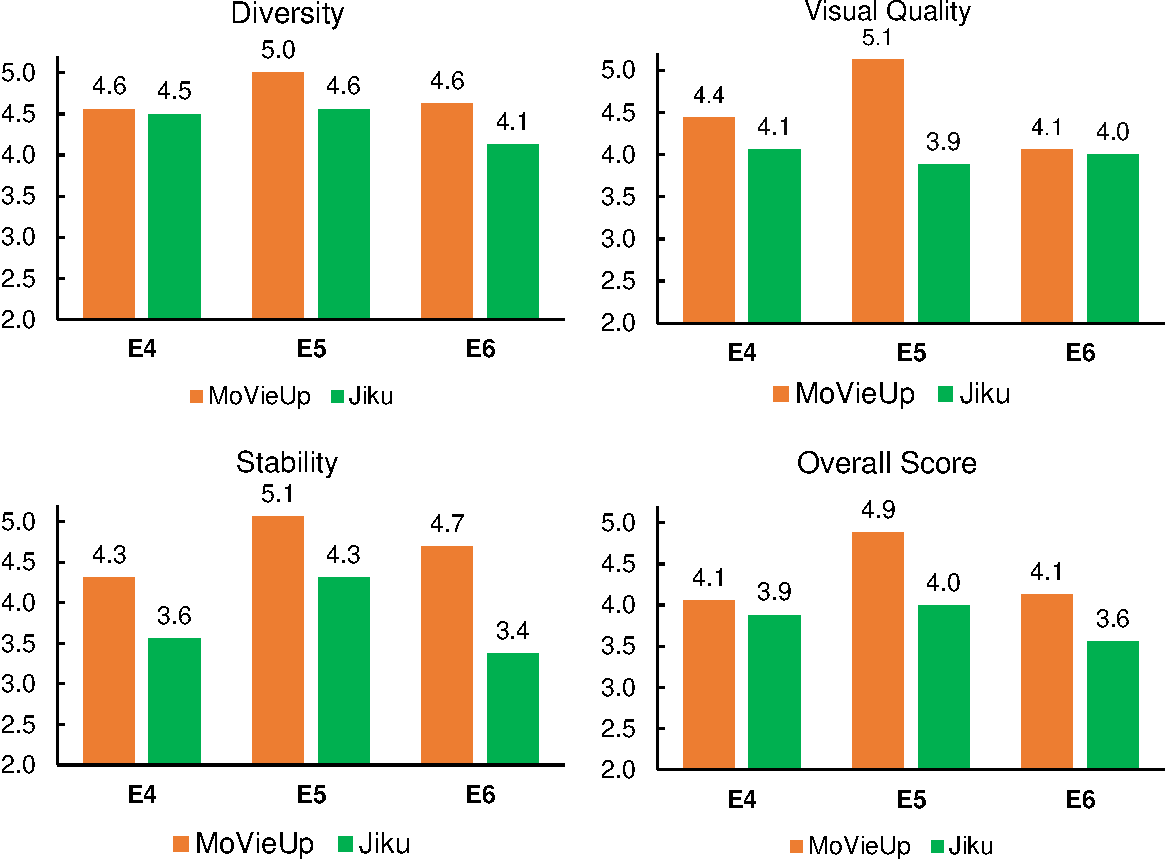
\includegraphics[clip=true, width=0.95\textwidth]{mashup-comp-jiku.pdf}
    \caption{MoVieUp系统与\emph{Jiku Director}的实验比较结果}
    \label{fig:mashup-comp-jiku}
\end{figure}

多样性方面,我们的系统获得了更好的效果,类似于与\emph{Virtual Director}的比较结果,
多样性方面的提升并不明显。两个系统都才用了基于关键帧的相似度方法,都采用了用户对内容
的兴趣随着镜头时长递减的多样性模型。多样性方面的区别在于\emph{Jiku Director}首先确定
镜头的视角(拍摄距离和角度),再从对应视角选取视频镜头。该策略可能使得连续视角比较接近
时降低多样性,与之对比,我们的系统根据一个记忆模型选取镜头。

对于视觉质量,连个系统在事件4和事件6四大行表现比较接近。系统均考虑了空间和时间上的
质量因素。我们采用了与\emph{Virtual Director}相同的客观比较方法对有问题的镜头进行标注,
结果如表格~\ref{tab:mashup-jiku-obj-comp}所示。虽然我们的系统在事件4上选取了更少的抖动
镜头,但选取了相对较多的失真镜头可能是导致视觉质量评分相差不大的主要因素。
在事件5中,MoVieUp系统表现要好得多。我们发现\emph{Jiku Director}产生的视频被遮挡,
强光和不规律的相机运动影响。对于事件6,编辑人员反应视频存在模糊问题。
根据图~\ref{tab:mashup-jiku-obj-comp}和表格~\ref{tab:mashup-jiku-obj-comp}的结果,
我们仍然可以总结出MoVieUp系统在视觉质量上比\emph{Jiku Director}表现更好。
\begin{table}[!t]
	\centering
    \caption{MoVieUp和\emph{Jiku Director}系统存在质量问题的镜头数量比较}
	\label{tab:mashup-jiku-obj-comp}
	\scriptsize
	\begin{tabular}{|c|c|c|c|c|c|c|}
		\hline
		\multirow{2}{*}{因素} & \multicolumn{3}{c|}{MoVieUp} &
		\multicolumn{3}{c|}{Jiku Director}  \\ \cline{2-7}
		& 事件4 & 事件5 & 事件6 & 事件4 & 事件5 & 事件6 \\ \hline
		镜头		& 49 & 21 & 37 & 49 & 26& 49 \\ \hline
		抖动	& 3 & 0 & 0 & 11 & 3& 3 \\ \hline
		过暗	& 1 & 0 & 0 & 0 & 0& 1 \\ \hline
		失真	& 5 & 1 & 1 & 7 & 3& 4 \\ \hline
	\end{tabular}
\end{table}

总结起来,本章提出的系统相对于已有的剪辑系统能达到更好的多样性,视觉质量和稳定性。
整体的评分表明能够该系统提供了更好的移动都摄像头视频观看体验。

\section{小结}
本章内容介绍了一个全自动移动多摄像头视频自动剪辑系统。该系统从多摄像头视频中剪辑
音频和视频,相比于已有的剪辑系统达到了更好的观看体验。系统基于从用户调研中得到的
电影语法。为了生成高质量的剪辑音频,系统对输入音频进行质量评估,并在\emph{最少切换准则}
下进行音频剪辑。在剪辑后的音频上,系统衡量节奏合适度和语义合适度,从而检测视频镜头的切换点。
对于视频镜头选取,系统考虑了相机运动一致性使得镜头平滑切换。为了保证视频质量,
系统考虑了空间和时间上的质量因素。为了增强内容的多样性,系统基于记忆模型解决视频的单调性问题。
视频剪辑最终通过优化问题进行求解。后处理操作进一步完善了剪辑视频的语义完整性,增加了视频
的稳定性。系统最后对剪辑音频和剪辑视频混流得到最后的剪辑结果。

本章的主要贡献包括:
\begin{itemize}
    \item 我们提出了全自动移动多摄像头自动剪辑系统,
        与已有系统需要一部分人工干预具有显著区别。
    \item 系统进行了电影语法的调研,并引入了一系列可计算的专业剪辑规则。
        这些可计算的语法提供了镜头切换和选取的指导规则。
    \item 除了视频剪辑,我们首次考虑了音频剪辑,并显著提高了多摄像头视频的观看体验。
        音频剪辑的作用经常被现有系统忽视,然而它对于提升用户体验十分重要。
\end{itemize}
